\newcolumntype{+}{>{\global\let\currentrowstyle\relax}}
\newcolumntype{^}{>{\currentrowstyle}}
\newcommand{\rowstyle}[1]{\gdef\currentrowstyle{#1}%
#1\ignorespaces
}

\newcommand{\specialcell}[2][c]{%
  \begin{tabular}[#1]{@{}c@{}}#2\end{tabular}}

\crefname{equation}{equation}{equations}
\Crefname{equation}{Equation}{Equations}% For beginning \Cref
\crefrangelabelformat{equation}{(#3#1#4--#5#2#6)}

\crefmultiformat{equation}{equations (#2#1#3}{, #2#1#3)}{#2#1#3}{#2#1#3}
\Crefmultiformat{equation}{Equations (#2#1#3}{, #2#1#3)}{#2#1#3}{#2#1#3}

\chapter{Experiments and Results}
\label{sec:exp}

This chapter presents the experiments and results of running the SAD algorithm on the FPGA board in comparison to running the algorithm on a general purpose CPU core. The code used on the FPGA board was written in VHDL and the code used on the CPU core was written in C. Disparity map images, testbench simulations, and counting clock cycles were used to compare the accuracy and speed of the VHDL implementations to the C implementation.

\section{Methodology}
\label{sec:method}

The experiments and results presented in this section used the FPGA Atlys board and a desktop computer that has an i7 CPU 950 at 3.07 GHz, 16 GB of RAM, and runs Ubuntu 64-bit. Due to hardware and timing issues with the DDR2 memory chip on the FPGA board, the board was unable to hold all of the data for both images. Part of the rows of both images were sent to the FPGA board from the computer. The board processed the data and sent the disparity values back to the computer. The computer then provided the board with the next set of partial row data and so on until the entire disparity map was created. The images were processed from top to bottom, left to right, where the column width was based on the number of pixels processed in parallel. This was used to test the quality and accuracy of the disparity maps from the FPGA implementation in comparison to computer implementation in C. The transfer time of sending both images to the FPGA board and getting back the disparity map was not a real-time solution since it took at least 20 seconds to complete the whole process. To test for the maximum possible frames per second the SAD wrapper could perform at, clock cycle counting on the FPGA board and testbench simulations were used to obtain the time it should take to produce a disparity map on the board for a 100 MHz clock. The Atlys board has a 100 MHz clock on it, which determined the clock cycle of 10 ns in the testbench simulations. However, for the experiments that produced the disparity image maps where the image data was sent from the computer to the board, a 48 MHz clock was used, which was the clock frequency of the FPGALink. This was done in order to synchronize the input data with the SAD wrapper. 

\section{Window Size Selection}
\label{sec:windowSize}

The size of the window (e.g. 9x9 pixels) affected the quality of the disparity map (see Figure~\ref{fig:tsukubaWinSize}) and the number of computations required to create the disparity map. The 3x3 window size used in Figure~\ref{fig:tsukuba3x3} was the fastest out of the window sizes shown since each SAD calculation only had 9 pairs of pixels to process. The 13x13 window in Figure~\ref{fig:tsukuba13x13} has 169 pairs of pixels, which required 160 more calculations per SAD value. However, the 13x13 window has the least amount of noise in its disparity map image, but it loses some detail as shown by comparing the neck of the lamp in the foreground of the image to the lamp necks in the other images. Table~\ref{table:pixelCount} shows the number of pixels needed based on the window size and the number of pixels processed in parallel. As the window size increased, more resources were needed on the FPGA board. The 7x7 and 9x9 window sizes were selected because they provided a good compromise on the amount of noise in the disparity maps to the amount of hardware resources required for implementation.

\begin{figure}
\begin{center}
	\begin{subfigure}{0.45\textwidth}
		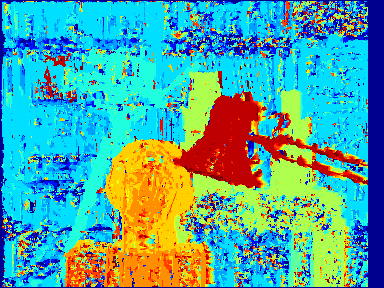
\includegraphics[width=\textwidth]{figures/sad_tsukuba_3x3_0-15.png}
		\caption{SAD 3x3 Window Disparity Map}
		\label{fig:tsukuba3x3}
	\end{subfigure}
	\begin{subfigure}{0.45\textwidth}
		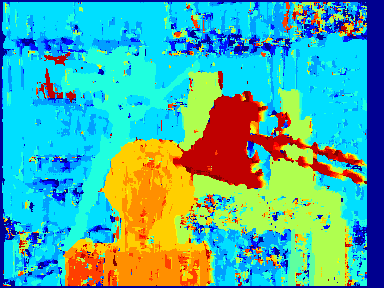
\includegraphics[width=\textwidth]{figures/sad_tsukuba_5x5_0-15.png}
		\caption{SAD 5x5 Window Disparity Map}
		\label{fig:tsukuba5x5}
	\end{subfigure}
	\\
	\begin{subfigure}{0.45\textwidth}
		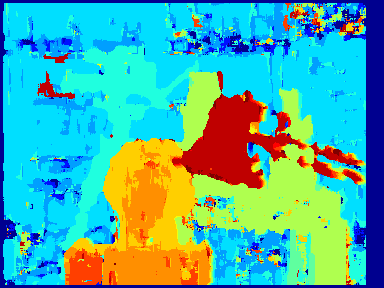
\includegraphics[width=\textwidth]{figures/sad_tsukuba_7x7_0-15.png}
		\caption{SAD 7x7 Window Disparity Map}
		\label{fig:tsukuba7x7}
	\end{subfigure}
	\begin{subfigure}{0.45\textwidth}
		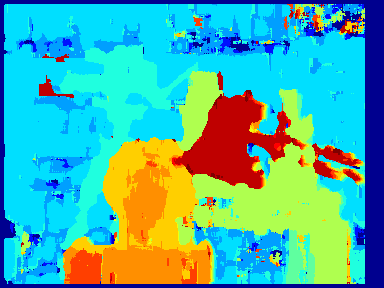
\includegraphics[width=\textwidth]{figures/sad_tsukuba_9x9_0-15.png}
		\caption{SAD 9x9 Window Disparity Map}
		\label{fig:tsukuba9x9}
	\end{subfigure}
	\\
	\begin{subfigure}{0.45\textwidth}
		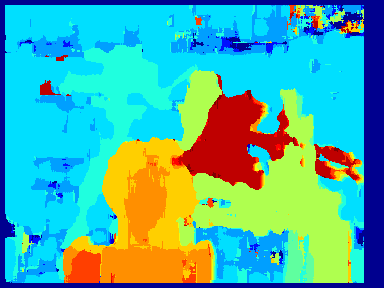
\includegraphics[width=\textwidth]{figures/sad_tsukuba_11x11_0-15.png}
		\caption{SAD 11x11 Window Disparity Map}
		\label{fig:tsukuba11x11}
	\end{subfigure}
	\begin{subfigure}{0.45\textwidth}
		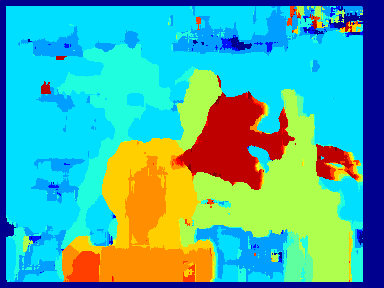
\includegraphics[width=\textwidth]{figures/sad_tsukuba_13x13_0-15.png}
		\caption{SAD 13x13 Window Disparity Map}
		\label{fig:tsukuba13x13}
	\end{subfigure}
	\captionfonts
	\caption{Window size comparisons for disparity maps~\cite{matlab} of the Tsukuba image pair~\cite{middlebury}.}
	\label{fig:tsukubaWinSize}
\end{center}
\end{figure}

\begin{table}
\begin{center}
	\begin{tabular}{| p{1.7cm} | p{2.5cm} | p{2.7cm} | >{\raggedright} p{2.7cm} | >{\raggedright\arraybackslash} p{2.7cm} |}
		\hline
		\rowstyle{\bfseries} Window Size & 
		\rowstyle{\bfseries} \# of pixels/ window & 
		\rowstyle{\bfseries} \# of pixels/ disparity value & 
		\rowstyle{\bfseries} \# of pixels/ 2 disparity values & 
		\rowstyle{\bfseries} \# of pixels/ 4 disparity values
		\tabularnewline
		\hline
		3x3 & 9 & 108 & 114 & 126
		\tabularnewline
		\hline
		5x5 & 25 & 200 & 210 & 230
		\tabularnewline
		\hline
		\rowstyle{\bfseries} 7x7 & 
		\rowstyle{\bfseries} 49 & 
		\rowstyle{\bfseries} 308 & 
		\rowstyle{\bfseries} 322 & 
		\rowstyle{\bfseries} 350
		\tabularnewline
		\hline
		\rowstyle{\bfseries} 9x9 & 
		\rowstyle{\bfseries} 81 & 
		\rowstyle{\bfseries} 432 & 
		\rowstyle{\bfseries} 480 & 
		\rowstyle{\bfseries} 486
		\tabularnewline
		\hline
		11x11 & 121 & 572 & 594 & 638
		\tabularnewline
		\hline
		13x13 & 169 & 728 & 754 & 806		
 		\tabularnewline
		\hline 
	\end{tabular}
	\captionfonts
	\caption{Number of 1 byte pixels based on the window size and number of pixels processed in parallel for producing disparity values simultaneously for a disparity range of 16.}
	\label{table:pixelCount}
\end{center}
\end{table}

\section{Resource Utilization on FPGA}
\label{sec:utilize}

The disparity range used to obtain the disparity value for each pixel affects the number of SAD entities and the number of minimum comparator entities required. Table~\ref{table:dispRange} shows the direct correlation between the disparity range and number of those entities needed. A lower disparity range of 8 requires fewer resources, but does not work well for objects that get close to the pair of cameras. A disparity range of 32 will give better results with objects that are closer; however, the resource requirements increase. The disparity range of 16 was selected since it provided a compromise of resource space to minimum detectable object distance. For a disparity range of 16, Table~\ref{table:pixelInParallel} shows the amount of SAD algorithm and minimum comparator entities needed to processing different numbers of pixels in parallel. Processing 2 or 4 pixels in parallel allowed for the speed needed while having a resource utilization size that fits on the Atlys board.

See Table~\ref{table:utilize} for resource utilization. The bold 7x7 and 9x9 rows were the resource utilization of the implementations presented in Chapter~\ref{sec:impl}. The bold 7x7 window implementation used slightly more resources on the FPGA board than the bold 9x9 window implementation due to the additional space requirements of the parallelized SAD algorithms. Both bold implementations used more resources than the other implementations of their same window size. The bold 7x7 implementation processed half the amount of pixels in parallel, but each of its SAD algorithm entities has 7 times as many subtracters than the other 7x7 implementation, which allowed it to run faster while taking up more space. The bold 9x9 implementation processed more pixels in parallel than the other 9x9 implementations and therefore needed more resources. There is plenty of space on the board for other top level entity designs for these SAD modules.

\begin{table}
\begin{center}
	\begin{tabular}{| p{2cm} | p{4cm} | p{5cm} |}
		\hline 
		\rowstyle{\bfseries} Disparity Range & 
		\rowstyle{\bfseries} \# of SAD entities/ pixel in parallel &
		\rowstyle{\bfseries} \# of Min. Comp. entities/ pixel in parallel
		\\ \hline
		8 & 8 & 7
		\\ \hline 
		\rowstyle{\bfseries} 16 & 
		\rowstyle{\bfseries} 16 & 
		\rowstyle{\bfseries} 15
		\\ \hline
		32 & 32 & 31
		\\ \hline 
	\end{tabular}
	\captionfonts
	\caption{Number of SAD algorithm entities and minimum comparators entities needed per pixel processed in parallel based on the disparity range.}
	\label{table:dispRange}
\end{center}
\end{table}

\begin{table}
\begin{center}
	\begin{tabular}{| p{3cm} | p{2.7cm} | p{3.7cm} |}
		\hline 
		\rowstyle{\bfseries} \# of pixels in parallel & 
		\rowstyle{\bfseries} \# of SAD entities &
		\rowstyle{\bfseries} \# of Min. Comp. entities 
		\\ \hline
		1 & 16 & 15
		\\ \hline 
		\rowstyle{\bfseries} 2 & 
		\rowstyle{\bfseries} 32 & 
		\rowstyle{\bfseries} 30
		\\ \hline 
		\rowstyle{\bfseries} 4 & 
		\rowstyle{\bfseries} 64 & 
		\rowstyle{\bfseries} 60
		\\ \hline
		6 & 96 & 90
		\\ \hline 
	\end{tabular}
	\captionfonts
	\caption{Number of SAD algorithm and minimum comparator entities needed based on the number of pixels processed in parallel for a disparity range of 16.}
	\label{table:pixelInParallel}
\end{center}
\end{table}

\begin{table}
\begin{center}
	\begin{tabular}{| p{1.9cm} | p{2.2cm} | p{2.5cm} | p{2.9cm} | p{2.7cm} |}
		\hline
		\rowstyle{\bfseries} Window Size & 
		\rowstyle{\bfseries} \# of pixels in parallel & 
		\rowstyle{\bfseries} SAD Alg. Parallelized & 
		\rowstyle{\bfseries} \# of Slice Registers, out of 54,576 &
		\rowstyle{\bfseries} \# of Slice LUTs, out of 27,288 %& 
		%\rowstyle{\bfseries} \# of occupied Slices, out of 6,822
		\tabularnewline
		\hline
		7x7 & 4 & No & 8,729 (15\%) & 12,215 (44\%)
		\tabularnewline
		\hline 
		\rowstyle{\bfseries} 7x7 & 
		\rowstyle{\bfseries} 2 & 
		\rowstyle{\bfseries} Yes & 
		\rowstyle{\bfseries} 10,990 (20\%) & 
		\rowstyle{\bfseries} 17,329 (63\%)  
		\tabularnewline
		\hline 
		\rowstyle{\bfseries} 9x9 & 
		\rowstyle{\bfseries} 4 & 
		\rowstyle{\bfseries} No & 
		\rowstyle{\bfseries} 10,969 (20\%) & 
		\rowstyle{\bfseries} 15,359 (56\%) 
		\tabularnewline
		\hline
		9x9 & 2 & No & 8,306 (15\%) & 12,414 (45\%)
		\tabularnewline
		\hline 
		9x9 & 1 & No & 7,108 (13\%) & 10,426 (38\%)
		\tabularnewline
		\hline 
	\end{tabular}
	\captionfonts
	\caption{Resource utilization on the FPGA Atlys board for different window implementations.}
	\label{table:utilize}
\end{center}
\end{table}

\section{Testbench Simulation}
\label{sec:testbench}

See Figure~\ref{fig:tb_9x9} and Figure~\ref{fig:tb_7x7} in Appendix~\ref{sec:appdxD} for the testbench simulations for the 9x9 window and 7x7 window implementations, respectively.

The signal h2fvalid\_i, near the top of the figures, went high when image data was sent to the SAD wrapper. For the 9x9 implementation, a cycle was created from the number of clock cycles it took for the SAD algorithms and minimum comparators to run. The signal data\_out went low when the SAD algorithms were running and went high after the SAD values were sent to the minimum comparators. For the 7x7 implementation with parallelized SAD, the SAD algorithms and minimum comparators finished in fewer clock cycles than it took to write in the next pair of row data. The cycle was created from the number of clock cycles it took to write in the row data. The SAD wrapper was designed to allow both the template image data and the search image data to be sent to the wrapper at the same time, if desired, thus reducing the amount of time taken to get all necessary data into the wrapper. When the signal f2hready\_i goes high, it meant the disparity values were sent out of the SAD wrapper.

For the testbench simulations, it was assumed that the data being sent to the SAD wrapper was supplied when the desired data was needed. So there was no delay to slow the process down. On a full FPGA implementation, the image data would be stored in the DDR2 memory chip on the Atlys board from the cameras and then sent to the SAD wrapper. According to Digilent, the DDR2 can run at up to an 800 MHz data rate~\cite{atlysBoard}. However, for reading data out of the DDR2, it takes around 22 to 32 clock cycles to begin receiving data after sending the read command to it~\cite{ug388}. By configuring the DDR2 as 2 64-bit bi-directional ports, each image would have its own port and data could be clumped together for 8 bytes of data being read from it at a time. Using several BRAMs within the FPGA chip as an intermediary buffer between the DDR2 and SAD wrapper while reading enough data from the DDR2 at a time should be sufficient to prevent timing delays.

The 9x9 window implementation has its next data rows buffered while the SAD algorithms were running. The SAD algorithms took longer to run than it did to fill up the next rows. This means there were several clock cycles that could be used if the incoming data was slower than ideal speeds.

The 7x7 window implementation with parallelized SAD, for its maximum speed, needed a pixel of data sent into the SAD wrapper every clock cycle. In the simulation, h2fvalid\_i was always high, showing that data was always being sent into it. 

%\subsection{9x9 Window Implementation Runtime}
%\label{sec:testbench9x9}
%
%Based on the testbench simulation in Figure~\ref{fig:tb_9x9} the simulated frames per second can be inferred for different image sizes. The simulation assumes the 100 MHz clock on the FPGA is used, which was the clock frequency on the Atlys board. The clock cycle duration is therefore 10 ns long.
%
%In the testbench simulation, the window size is 9x9 and 4 pixels are processed in parallel. The first section of the simulation includes the initial image data given to the SAD wrapper up to the point where that data's disparity values are returned. This section takes 3.35 us. After that, a constant cycle was produced, which includes the SAD wrapper taking in the next row and producing the next disparity values. This cycle takes 1.22 us. A 640x480 image has 307,200 pixels, which will produce a disparity map of 617x472, or 291,224 pixels. Disparity values are not produced for pixels where either the window would run off the image or where there is not enough room for the 16 SAD values to be calculated for the pixel. Since 4 pixels are processed in parallel, 291,224 pixels are divided by 4 pixels/iteration, giving 72,806 iterations. So, 72,805 iterations times 1.22 us/iteration plus 3.35 us (initial section, hence minus one on number of iterations) gives 88,826.67 us or approximately 0.0888 seconds per frame. Therefore, an image size of 640x480 can be processed at around 11.26 frames per second. Table~\ref{table:tb_9x9} shows the simulated frame rate for the image sizes used in this chapter.
%
%\begin{table}
%	\begin{center}
%		\begin{tabular}{|c|c|c|c|c|}
%			\hline 
%				\rowstyle{\bfseries} Image & 
%				\rowstyle{\bfseries} Image Width & 
%				\rowstyle{\bfseries} Image Height & 
%				\rowstyle{\bfseries} Sec/frame & 
%				\rowstyle{\bfseries} Frames/sec
%			\tabularnewline
%			\hline 
%			Tsukuba & 384 & 288 & 0.02228 & 44.87
%			\tabularnewline
%			\hline 
%			Venus & 434 & 383 & 0.03359 & 29.77			
%			\tabularnewline
%			\hline 
%			VmodCAM & 640 & 480 & 0.06356 & 15.73
%			\tabularnewline
%			\hline 			
%			\end{tabular}
%		\captionfonts
%		\caption{9x9 window for the testbench simulated runtime for the FPGA board for different image sizes.}
%		\label{table:tb_9x9}
%	\end{center}
%\end{table}
%
%\subsection{7x7 Window Implementation Runtime}
%\label{sec:testbench7x7}
%
%Based on the testbench simulation in Figure~\ref{fig:tb_7x7} the simulated frame rate can be inferred for different image sizes. The simulation uses a clock cycle of 10 ns.
%
%In the testbench simulation, the window size is 7x7 and 2 pixels are processed in parallel. The first section of the simulation includes the initial image data given to the SAD wrapper up to the point where that data's disparity values are returned. This section takes 1.78 us. After that, a constant cycle is produced allowing the SAD wrapper to get the next row and produce the next disparity values, which takes 0.42 us. A 640x480 image has 307,200 pixels, which will produce a disparity map of 474x618, which is 292,932 pixels. Disparity values are not produced for pixels that either the windows cannot fit on or there is not enough room for the 16 SAD values to be calculated for the pixel. Since 2 pixels are processed in parallel, 292,932 pixels is divided by 2 pixels/iteration, giving 146,703 base iterations. There is an additional 1,848 iterations that occur due to the loading of the 6 top row segments  before any disparity values can be obtained for each column of the pair of pixels processed in parallel. There are 308 columns past the initial column (618/2 - 1) times 6 plus the base number of iterations gives a total of 148,551 iterations. The additional iterations causes an overhead of only 1.24\%. So, 148,551 total iterations times 0.24 us/iteration gives 61,617.04 us or approximately 0.0616 seconds per frame. Therefore, an image size of 640x480 can be processed at around 16.23 frames per second. Table~\ref{table:tb_7x7} shows the simulated frame rate for the image sizes used in this chapter.


%In the testbench simulation, the window size is 7x7 and 2 pixels are processed in parallel. The first section of the simulation includes the initial image data given to the SAD wrapper up to the point where that data's disparity values are returned. This section takes 1.78 us. After that, a constant cycle is produced allowing the SAD wrapper to get the next row and produce the next disparity values, which takes 0.42 us. A 640x480 image has 307,200 pixels, which will produce a disparity map of 619x474, which is 293,406 pixels. Disparity values are not produced for pixels that either the windows cannot fit on or there is not enough room for the 16 SAD values to be calculated for the pixel. Since 2 pixels are processed in parallel, 293,406 pixels is divided by 2 pixels/iteration, giving 146,703 iterations. So, 146,702 iterations times 0.42 us/iteration plus 1.78 us (initial section, hence minus one on number of iterations) gives 61,617.04 us or approximately 0.0616 seconds per frame. Therefore, an image size of 640x480 can be processed at around 16.23 frames per second. Table~\ref{table:tb_7x7} shows the simulated frame rate for the image sizes used in this chapter.

%\begin{table}
%	\begin{center}
%		\begin{tabular}{|c|c|c|c|c|}
%			\hline
%				\rowstyle{\bfseries} Image & 
%				\rowstyle{\bfseries} Image Width & 
%				\rowstyle{\bfseries} Image Height & 
%				\rowstyle{\bfseries} Sec/frame & 
%				\rowstyle{\bfseries} Frames/sec
%			\\ \hline 
%			Tsukuba & 384 & 288 & 0.01199 & 83.42
%			\\ \hline 
%			Venus & 434 & 383 & 0.01815 & 55.11
%			\\ \hline 
%			VmodCAM & 640 & 480 & 0.03411 & 29.32
%			\\ \hline 
%		\end{tabular}	
%		\captionfonts
%		\caption{7x7 window for the testbench simulation runtime for the FPGA board for different image sizes.}
%		\label{table:tb_7x7}
%	\end{center}
%\end{table}

\section{Pixel Parallelization}
\label{sec:7x7pixelParallel4}

The 7x7 window implementation used a parallelized SAD algorithm (see Section~\ref{sec:7x7window}). Due to the additional resources needed, only 2 pixels were processed in parallel instead of 4. The reduced number of pixels in parallel was made up for from the speed up of the SAD algorithm. In order to verify the parallelized SAD algorithm produced a speed up greater than reduction of pixels processed in parallel, a 7x7 window implementation of the 9x9 window implementation (see Section~\ref{sec:9x9window}) was introduced. This version of the 7x7 implementation processed 4 pixels in parallel (4 pix //) and its SAD algorithms were not parallelized.

\section{FPGA Clock Cycle Runtimes}

A clock cycle counter was introduced to 3 implementations, the 9x9 with 4 pixels in parallel, the 7x7 with 2 pixels in parallel and parallel SAD algorithms, and the 7x7 with 4 pixels in parallel (4 pix //). The 7x7 (4 pix //) was tested to demonstrate how the 7x7 with 2 pixels in parallel has a higher frame rate due to the parallelized SAD algorithms. 

Table~\ref{table:clockCount} shows the recorded clock cycle counts for the Tsukuba (384x288) and Venus (434x383) image pairs for the SAD algorithms and minimum comparators. The VmodCAM (640x480) clock cycles were calculated based on the series of equations in Equation~\ref{eq:clockCycles}. For all implementations, the minimum comparators took 4 clock cycles from when it got the 16 SAD values to when it output the disparity value for the lowest SAD value. The 7x7 with parallelized SAD has additional clock cycles due to how fast its SAD algorithms ran in comparison to data load times of the next row into the SAD wrapper.

Eq.~\ref{eq:clockCycles} produced the same SAD Cycles and Min. Comp. Cycles as the values recorded from the FPGA in Table~\ref{eq:clockCycles} for the Tsukuba and Venus image pairs. Eq.~\ref{eq:clockCycles} also was used to calculate the total cycles required per iteration. Testbench simulations in Appdx.~\ref{sec:appdxD} were used to determine the additional clock cycles needed per iteration. The simulations also verified the number of clock cycles required for data input, SAD algorithm, and minimum comparators.

~\Cref{eq:a,eq:b,eq:c,eq:d,eq:e,eq:f,eq:g} are the parameters for the rest of the equations. ~\Cref{eq:h} gives the height of the disparity map image. The width of the disparity map image, ~\Cref{eq:j}, needs to be divisible by ~\Cref{eq:e}, so ~\Cref{eq:i} is used to reduce it to a divisible amount. The number of pixels in the disparity map image is calculated in ~\Cref{eq:k}. The base number of iterations, ~\Cref{eq:l}, is the minimum number of iterations required to create the disparity map. Additional iterations, ~\Cref{eq:n}, occur from the SAD algorithm proceeding through the images in the form of columns, top to bottom, left to right. There are a certain amount of iterations at the top of each column that are not used because a winSize of rows must be loaded in order to obtain the disparity values. ~\Cref{eq:o} is the total number of iterations needed to process the pair of images. ~\Cref{eq:p} is the total number of cycles for the SAD algorithms. ~\Cref{eq:q} is the total number of cycles for the minimum comparators. ~\Cref{eq:r} represents the extra cycles that occur only for the 7x7 implementation with the parallelized SAD algorithms. For that implementation, the SAD algorithm is faster than the data can be loaded, so its iterations take longer than just the number of SAD algorithm and minimum comparator cycles. ~\Cref{eq:s} is the total number of cycles for the entire pair of images to be processed on the FPGA.

The 9x9 implementation was able to have its next rows of 27 pixels each buffered within the 82 clock cycles it took for the SAD algorithms to finish. There were a total of 86 clock cycles per iteration.

The 7x7 implementation with parallelized SAD was unable to have its next rows, 23 pixels each, buffered within the 8 clock cycles it took for the SAD algorithms to finish. The limiting factor was the time it took to buffer each pair of rows, so there were 23 clock cycles per iteration. The 4 clock cycles for the minimum comparators was hidden within the 23 clock cycles.

The 7x7 (4 pix //) implementation was able to have its next rows of 25 pixels each buffered within the 50 clock cycles it took for the SAD algorithms to finish. There were a total of 54 clock cycles per iteration.

Table~\ref{table:clockCountFPS} is a continuation of Table~\ref{table:clockCount}. It shows the time it took to process a frame and the frame rate with a clock speed of 48 MHz and 100 MHz. The 48 MHz was the transfer rate of the FPGALink between the computer and the FPGA board. It was used in order to not introduce timing issues for the data given to the SAD wrapper. The image processing on the FPGA board always takes a consistent amount of clock cycles, relative to the image sizes, so the frame rate can be calculated for a clock speed of 100 MHz, which is the clock frequency of the clock on the Atlys board.\\\\\\\\\\

\begin{subequations}
\begin{align}
	height = 288 	\qquad & \text{(image height)} \label{eq:a}\\
	width = 384 	\qquad & \text{(image width)} \label{eq:b}\\
	winSize = 9	 	\qquad & \text{(9x9 window size)} \label{eq:c}\\
	dispRange = 16 	\qquad & \text{(disparity range 0-15)} \label{eq:d}\\
	parPix = 4 		\qquad & \text{(pixels processed in parallel)} \label{eq:e}\\
	sadCyc = 82		\qquad & \text{(\# of cycles for SAD algorithm)} \label{eq:f}\\
	minCyc = 4		\qquad & \text{(\# of cycles for minimum comparator)} \label{eq:g}\\ 
	\nonumber\\
	dispH = 280 &= height - (winSize - 1) \label{eq:h}\\
	lessPix = 23 &= (dispRange-1) + (winSize-1) \label{eq:i}\\
	dispW = 360 &= (width-lessPix) - (width-lessPix) \% parPix \label{eq:j}\\
	dispPixels = 100,800 &= dispH * dispW \label{eq:k}\\
	baseIters = 25,200 &= dispPixels / parPix \label{eq:l}\\
	colAdd = 89 &= dispWidth / parPix - 1 \label{eq:m}\\
	addIters = 712 &= colAdd * (winSize-1) \label{eq:n}\\
	totIters = 25,912 &= basIters + addIters \label{eq:o}\\
	sadTotCyc = 2,124,784 &= sadCyc * totIters \label{eq:p}\\
	minTotCyc = 103,648 &= minCyc * totIters \label{eq:q}\\
	extraCyc = 0 &= totIters * 0 \label{eq:r}\\
	totClkCyc = 2,228,432 &= sadTotCyc + minTotCyc + extraCyc \label{eq:s}
\end{align}
	\label{eq:clockCycles}
\end{subequations}

\begin{table}
	\begin{center}
		\begin{tabu}{| p{1.5cm} | p{1.9cm} | p{1,7cm} | p{1.7cm} | p{1.7cm} | p{1.5cm} | p{1.6cm} |}
			\hline
				\rowstyle{\bfseries} Image Size (WxH) & 
				\rowstyle{\bfseries} Disparity Image Size & 
				\rowstyle{\bfseries} Window Size & 
				\rowstyle{\bfseries} SAD Cycles & 
				\rowstyle{\bfseries} Min. Comp. Cycles &
				\rowstyle{\bfseries} Extra Cycles &
				\rowstyle{\bfseries} Total Clock Cycles			
			\\ \hline 
			384x288 & 360x280 & 9x9 & 2,124,784 & 103,648 & 0 & 2,228,432
			\\ \hline 
			384x288 & 362x282 & 7x7 & 416,976 & 208,488 & 573,342 & 1,198,806
			\\ \hline 
			384x288 & 360x282 & \specialcell{7x7\\(4 pix //)} & 1,295,700 & 103,656 & 0 & 1,399,356
			\\ \tabucline[2pt]{-} 
			
			434x383 & 408x375 & 9x9 & 3,202,756 & 156,232 & 0 & 3,358,988
			\\ \hline 
			434x383 & 412x377 & 7x7 & 631,136 & 315,568 & 867,812 & 1,814,516
			\\ \hline 
			434x383 & 412x377 & \specialcell{7x7\\(4 pix //)} & 1,972,150 & 157,772 & 0 & 2,129,922
			\\ \tabucline[2pt]{-}
			
			640x480 & 616x472 & 9x9 & 6,060,784 & 295,648 & 0 & 6,356,432
			\\ \hline 
			640x480 & 618x474 & 7x7 & 1,186,512 & 593,256 & 1,631,454 & 3,411,222
			\\ \hline 
			640x480 & 616x474 & \specialcell{7x7\\(4 pix //)} & 3,695,700 & 295,656 & 0 & 3,991,356
			\\ \hline
		\end{tabu}	
		\captionfonts
		\caption{Number of clock cycles counted when a pair of images were processed on the FPGA for the SAD algorithms and the minimum comparators.}
		\label{table:clockCount}
	\end{center}
\end{table}

%\renewcommand{\arraystretch}{1.5}
\begin{table}
	\begin{center}
		\begin{tabu}{| p{1.8cm} | p{1.8cm} | p{2cm} | p{2cm} | p{2cm} | p{2cm} |}
			\hline
				\rowstyle{\bfseries} Window Size & 
				\rowstyle{\bfseries} Total Cycles & 
				\rowstyle{\bfseries} Sec/ Frame @ 48 MHz & 
				\rowstyle{\bfseries} Sec/ Frame @ 100 MHz & 
				\rowstyle{\bfseries} Frames/ Sec @ 48 MHz &
				\rowstyle{\bfseries} Frames/ Sec @ 100 MHz 
			\\ & & & & &\tabularnewline %[.01ex]
			\hline 
			9x9 & 2,228,432 & 0.04642 & 0.02228 & 21.54 & 44.87
			\\ \hline 
			7x7 & 1,198,806 & 0.02497 & 0.01199 & 40.05 & 83.42
			\\ \hline 
			\specialcell{7x7\\(4 pix //)} & 1,399,356 & 0.02915 & 0.01399 & 34.31 & 71.46
			\\ \tabucline[2pt]{-} 
			
			9x9 & 3,358,988 & 0.06997 & 0.03359 & 14.29 & 29.77
			\\ \hline 
			7x7 & 1,814,516 & 0.03780 & 0.01815 & 26.46 & 55.11
			\\ \hline 
			\specialcell{7x7\\(4 pix //)} & 2,129,922 & 0.04437 & 0.02130 & 22.54 & 46.95
			\\ \tabucline[2pt]{-}
			
			9x9 & 6,356,432 & 0.1324 & 0.06356 & 7.553 & 15.73
			\\ \hline 
			7x7 & 3,411,222 & 0.06578 & 0.03411 & 14.07 & 29.32
			\\ \hline 
			\specialcell{7x7\\(4 pix //)} & 3,991,356 & 0.08314 & 0.03991 & 12.03 & 25.05
			\\ \hline
		\end{tabu}	
		\captionfonts
		\caption{Frame rates that are possible for the number of clock cycles taken per image.}
		\label{table:clockCountFPS}
	\end{center}
\end{table}

\subsection{Frame Rate}
\label{sec:frameRate}

The smaller the image size, the higher the frame rate, as shown in Figure~\ref{fig:frameRate}. Once the number of pixels in an image goes below 300,000 for the 7x7 window implementation or 170,000 for the 9x9 window implementation, the frame rate reaches 30 frames per second. For robots, a frame rate of 10 should be sufficient for most tasks. Both the 9x9 and 7x7 window implementations were shown be above 10 frames per second for an image size of 640x480. Therefore it is possible to use larger image sizes and still get at least 10 frames per second.

\begin{figure}
	\begin{center}
		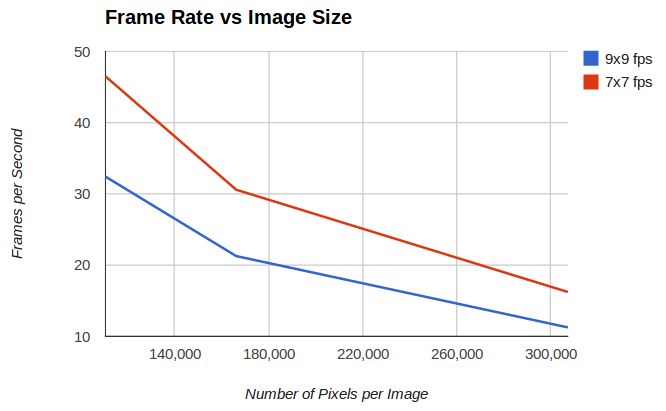
\includegraphics[width=100mm]{figures/frameRate.png}
		\captionfonts
		\caption{Frame rate comparison of different image sizes.}
		\label{fig:frameRate}
	\end{center}
\end{figure}

\section{Test Image Pairs}
\label{sec:runtime}

In this section, FPGA disparity maps were compared to disparity maps created using C code. Part of the SAD algorithm implementation in C is shown in Appendix~\ref{sec:appdxE}. The C SAD version was performed completely in serial, so 1 pixel was processed at a time. The images the C version produced were used to compare disparity map quality and runtime of the VHDL algorithm for the FPGA board. Python was used to convert the grayscale images into text files. Each row was separated by a new line. Each column was separated by a blank space. The C code read in the data from the text files, performed the SAD algorithm on the data, and wrote the disparity map data to a text file. The disparity map text file was read by another Python script and converted into a disparity map image. The time comparisons focused on the total time it took the SAD algorithm to run and disparity map data to be generated from the SAD values.

Table~\ref{table:runtimeComp} shows the frames per second (FPS) comparisons for the Tsukuba and Venus image pairs between C and VHDL implementations. The C code was compiled with gcc using optimization O2 and ran on a single processor core. The 7x7 window implementation with parallelized SAD and 9x9 window implementation are the 7x7 and 9x9 shown for the VHDL code in the table. The 7x7 VHDL implementation averaged around 12.80 times faster than the C 7x7 version. The 9x9 VHDL implementation was around 11.12 times faster than the C 9x9 version.

\begin{table}
	\begin{center}
		\begin{tabu}{|c|c|c|c|c|c|}
			\hline
				\rowstyle{\bfseries} Image & 
				\rowstyle{\bfseries} Window Size & 
				\rowstyle{\bfseries} Code & 
				\rowstyle{\bfseries} Sec/frame & 
				\rowstyle{\bfseries} FPS &
				\rowstyle{\bfseries} Speed up
			\\ \hline 
			Tsukuba & 7x7 & C & 0.1532 & 6.527 & 1
			\\ \hline 
			Tsukuba & 7x7 & VHDL & 0.01199 & 83.42 & 12.78
			\\ \tabucline[2pt]{-}
			Tsukuba & 9x9 & C & 0.2454 & 4.075 & 1
			\\ \hline 
			Tsukuba & 9x9 & VHDL & 0.02228 & 44.87 & 11.01
			\\ \tabucline[2pt]{-}
			Venus & 7x7 & C & 0.2327 & 4.297 & 1
			\\ \hline 
			Venus & 7x7 & VHDL & 0.01815 & 55.11 & 12.83
			\\ \tabucline[2pt]{-}
			Venus & 9x9 & C & 0.3776 & 2.648 & 1
			\\ \hline 
			Venus & 9x9 & VHDL & 0.03359 & 29.77 & 11.24
			\\ \hline 
		\end{tabu}	
		\captionfonts
		\caption{Tsukuba and Venus image pairs comparison runtimes for C code and FPGA testbench simulations. The disparity range is 16 for both.}
		\label{table:runtimeComp}
	\end{center}
\end{table}

\subsection{Data Overflows}
\label{sec:overflow}

The size of the data used for storing logic and values in hardware was defined during the coding process. In the SAD algorithm, it was possible for the SAD value to become much greater than the individual pixel values. For example, the pixel values range from 0 to 255, or 8 bits, while some SAD values could be over 4,095 and need to be stored in more than 12 bits. Most SAD values were under 4,096, so the SAD algorithm used 14 bits to account for any values from 0 to 16,383. Figure~\ref{fig:overflow} shows what can happen when the data size allotted for the SAD algorithm was not large enough (e.g. only having 10 bits for storage). The data used was unsigned, so when it went above the highest supported value, it went back down to 0 and continued from there.

Since most of the values were below 4,096, a measure was put in place to reduce the amount of bits needed during the minimum comparisons. If a SAD value was greater than 4,095, then 4,095 was returned for that calculated SAD value because the greater that the value is the less likely that search pixel will be the matching pixel to the corresponding template pixel. In Figure~\ref{fig:tsukubaDispMap} and Figure~\ref{fig:venusDispMap}, there are a total of 64 pixels that differ between all of the disparity map images. All of the differing pixels were in the 9x9 Venus disparity image, which were from those SAD values being over 4,095 and were handled accordingly. In the disparity map images, the objects closer to the cameras have a warmer color while objects farther away have a cooler color. %The colors show that warmer is closer and cooler is farther away. %For a robot, it would be better to error on the side of thinking an object is closer than it actually is because the robot will be less prone to collide with the object. If a robot thought an object was farther away than it actually was, then the likelihood of collision would increase.

\begin{figure}[h]
	\begin{center}
		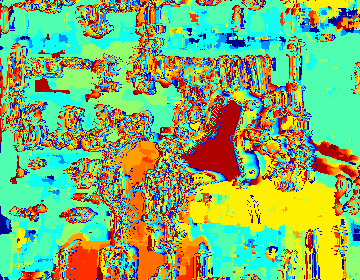
\includegraphics[width=80mm]{figures/tsukuba_disp9x9_2_sad_overflow.png}
		\captionfonts
		\caption{Data overflow for Tsukuba image pair~\cite{middlebury}.}
		\label{fig:overflow}
	\end{center}
\end{figure}

\subsection{Tsukuba}
\label{sec:tsukuba}

In Figure~\ref{fig:tsukubaL} and Figure~\ref{fig:tsukubaR}, the Tsukuba image pair is shown. Figure~\ref{fig:tsukubaDispMap} shows how the 7x7 window implementation is slightly noisier than the 9x9 window implementation. There were no differences between the corresponding disparity maps of the C code to the VHDL code.

%For Tsukuba, the FPGA version has a simulated runtime of 32.43 and 46.51 frames per second for the 9x9 and 7x7 window implementations, respectively, from Table~\ref{table:tb_9x9} and Table~\ref{table:tb_7x7}. For a speed comparison, the SAD algorithm was implemented in C since it is faster than Python. Python code handled the code for reading the images and creating the disparity map. As shown in Table~\ref{table:runtimeComp}, the C code processed the images serially, which took 1.4128 seconds for the 9x9 window with a disparity range of 16. The 7x7 window implementation in C with a disparity range of 16 took 0.8849 seconds to complete.


\subsection{Venus}
\label{sec:venus}

In Figure~\ref{fig:venusL} and Figure~\ref{fig:venusR}, the Venus image pair is shown. In the image pair, the newspaper articles are flat and slanted, relative to the cameras. This gradual slope, also present in the background, can be difficult for the SAD algorithm to deal with; however, the algorithm was able to give a fairly accurate representation of the depth in the image. It also caused the gradient pattern shown in the disparity maps. The 7x7 window depth maps have more noise than the 9x9 window depth maps. The only difference between the corresponding disparity maps of the C code to the VHDL code were with the 9x9 implementations. There were 64 pixels that differed between the C and FPGA 9x9 implementations. The SAD values that correspond to those pixels on the FPGA were above 4,095, so they were cut off at 4,095. The 64 pixels out of 155,324 pixels only gives 0.0412\% error.


\subsection{Cones}
\label{sec:cones}

In Figure~\ref{fig:conesL} and Figure~\ref{fig:conesR}, the Cones image pair is shown. Figure~\ref{fig:conesDispMap} shows the issue of objects being too close to the stereo cameras. The closer an object is to the stereo cameras, the greater its disparity value is and the greater the disparity range needs to be. Using the SAD algorithm with a 9x9 window and a disparity range of 60 (as opposed to the range of 16 used on the FPGA board) produces the results in Figure~\ref{fig:conesMatlab}. When the disparity range is not high enough, the disparity map in Figure~\ref{fig:conesPy} is produced.



\begin{figure}
\begin{center}
	\begin{subfigure}{0.45\textwidth}
		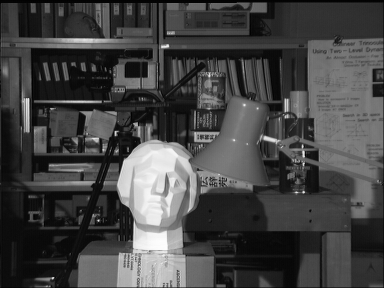
\includegraphics[width=\textwidth]{figures/tsukubaL.jpg}
		\caption{Left Tsukuba Grayscale Image}
		\label{fig:tsukubaL}
	\end{subfigure}
	\begin{subfigure}{0.45\textwidth}
		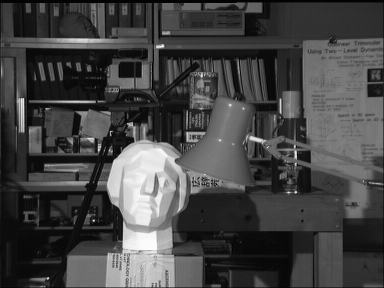
\includegraphics[width=\textwidth]{figures/tsukubaR.jpg}
		\caption{Right Tsukuba Grayscale Image}
		\label{fig:tsukubaR}
	\end{subfigure}
	\\
	\begin{subfigure}{0.45\textwidth}
		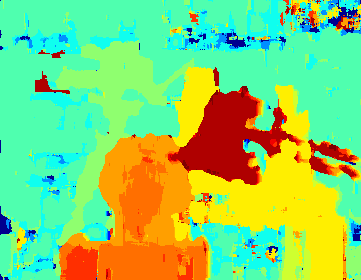
\includegraphics[width=\textwidth]{figures/tsukuba_c_9x9.png}
		\caption{C 9x9 Disparity Map}
		\label{fig:tsukubaC9x9}
	\end{subfigure}
	\begin{subfigure}{0.45\textwidth}
		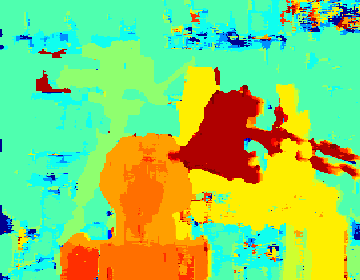
\includegraphics[width=\textwidth]{figures/tsukuba_buffer_9x9_4.png}
		\caption{FPGA 9x9 Disparity Map}
		\label{fig:tsukubaFPGA9x9}
	\end{subfigure}
	\\
	\begin{subfigure}{0.45\textwidth}
		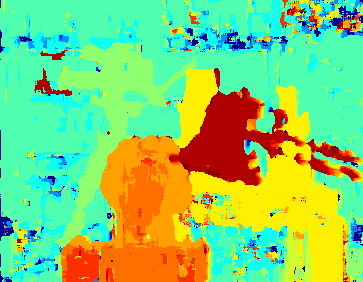
\includegraphics[width=\textwidth]{figures/tsukuba_c_7x7.png}
		\caption{C 7x7 Disparity Map}
		\label{fig:tsukubaC7x7}
	\end{subfigure}
	\begin{subfigure}{0.45\textwidth}
		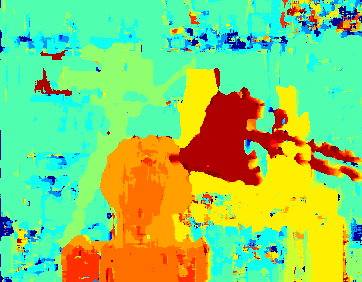
\includegraphics[width=\textwidth]{figures/tsukuba_buffer_7x7_2.png}
		\caption{FPGA 7x7 Disparity Map}
		\label{fig:tsukubaFPGA7x7}
	\end{subfigure}
	\captionfonts
	\caption{Disparity map comparison of the Tsukuba image pair~\cite{middlebury}.}
	\label{fig:tsukubaDispMap}
\end{center}
\end{figure}


\begin{figure}
\begin{center}
	\begin{subfigure}{0.45\textwidth}
		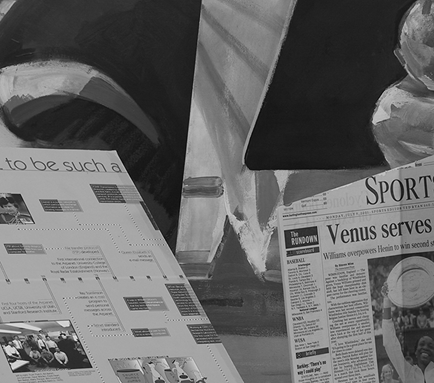
\includegraphics[width=\textwidth]{figures/venusL.png}
		\caption{Left Venus Grayscale Image}
		\label{fig:venusL}
	\end{subfigure}
	\begin{subfigure}{0.45\textwidth}
		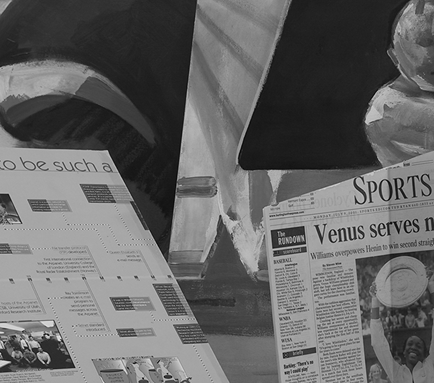
\includegraphics[width=\textwidth]{figures/venusR.png}
		\caption{Right Venus Grayscale Image}
		\label{fig:venusR}
	\end{subfigure}
	\\
	\begin{subfigure}{0.45\textwidth}
		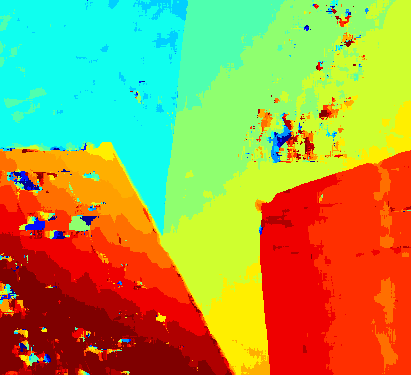
\includegraphics[width=\textwidth]{figures/venus_c_9x9.png}
		\caption{C 9x9 Disparity Map}
		\label{fig:venusC9x9}
	\end{subfigure}
	\begin{subfigure}{0.45\textwidth}
		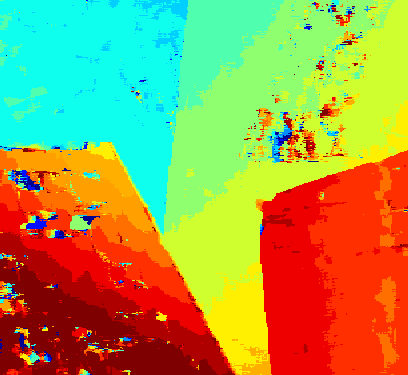
\includegraphics[width=\textwidth]{figures/venus_buffer_9x9_4.png}
		\caption{FPGA 9x9 Disparity Map}
		\label{fig:venusFPGA9x9}
	\end{subfigure}
	\\
	\begin{subfigure}{0.45\textwidth}
		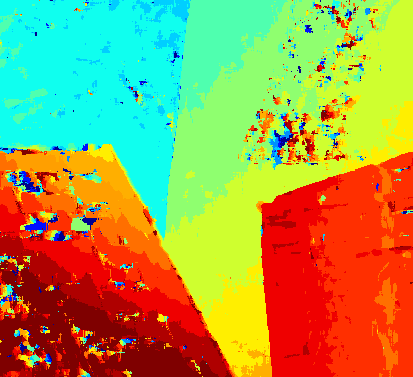
\includegraphics[width=\textwidth]{figures/venus_c_7x7.png}
		\caption{C 7x7 Disparity Map}
		\label{fig:venusC7x7}
	\end{subfigure}
	\begin{subfigure}{0.45\textwidth}
		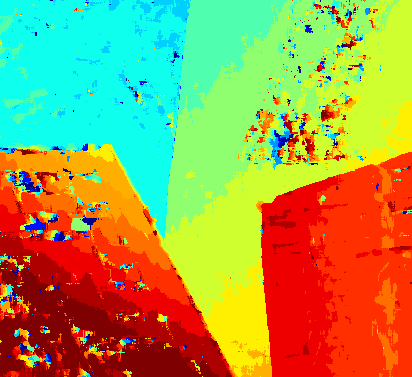
\includegraphics[width=\textwidth]{figures/venus_buffer_7x7_2.png}
		\caption{FPGA 7x7 Disparity Map}
		\label{fig:venusFPGA7x7}
	\end{subfigure}
	\captionfonts
	\caption{Disparity map comparison of the Venus image pair~\cite{middlebury}.}
	\label{fig:venusDispMap}
\end{center}
\end{figure}



\begin{figure}
\begin{center}
	\begin{subfigure}{0.45\textwidth}
		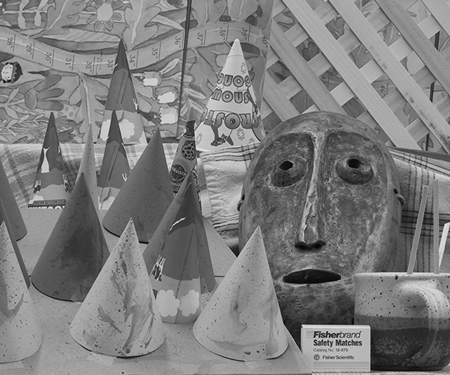
\includegraphics[width=\textwidth]{figures/conesL.png}
		\caption{Left Cones Grayscale Image}
		\label{fig:conesL}
	\end{subfigure}
	\begin{subfigure}{0.45\textwidth}
		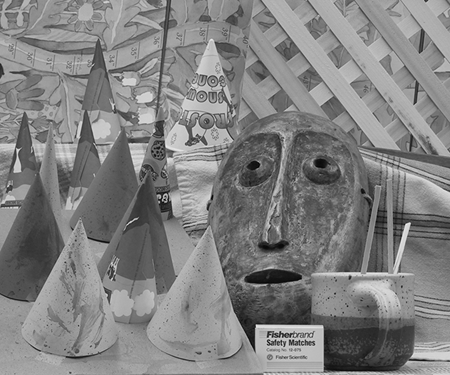
\includegraphics[width=\textwidth]{figures/conesR.png}
		\caption{Right Cones Grayscale Image}
		\label{fig:conesR}
	\end{subfigure}
	\\
	\begin{subfigure}{0.45\textwidth}
		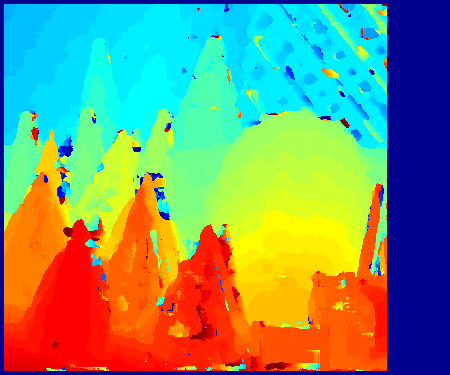
\includegraphics[width=\textwidth]{figures/cones_9x9_matlab_0-59.png}
		\caption{9x9 at Disparity Range of 60 ~\cite{matlab}}
		\label{fig:conesMatlab}
	\end{subfigure}
	\begin{subfigure}{0.45\textwidth}
		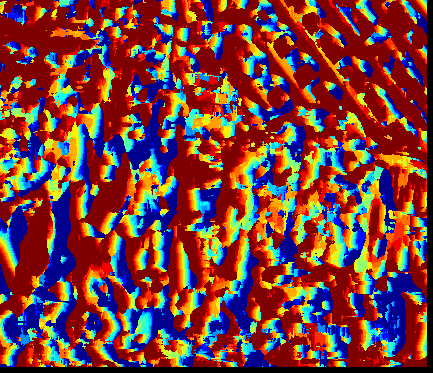
\includegraphics[width=\textwidth]{figures/cones_9x9_python3.png}
		\caption{9x9 at Disparity Range of 16}
		\label{fig:conesPy}
	\end{subfigure}
	\captionfonts
	\caption{Disparity map comparison of the Cones image pair ~\cite{middlebury}.}
	\label{fig:conesDispMap}
\end{center}
\end{figure}




